% ================================================================
% SECTION 5: EMPIRICAL RESULTS (FGCS version: consolidated figures,
% Ethereum figures recomputed with corrected era boundaries and $/MiB units)
% ================================================================

This section presents our findings from 90~days of production data, organized by metric.

\subsection{Observation Window and Protocol Eras}
\label{sec:results-eras}

Our window (November~15, 2025 to February~14, 2026) contains several parameter changes that we treat as natural experiments:
\squishlist
    \item \textbf{Ethereum}: four regimes: Pectra (target~6/max~9 blobs), Fusaka (same blob parameters, plus PeerDAS and the EIP-7918 fee floor, from Dec~3), BPO1 (target~10/max~15, from Dec~9), and BPO2 (target~14/max~21, from Jan~7).
    \item \textbf{Celestia}: app version~6 from Nov~24, and a maximum-square increase from 128 to 256 (8 to 32~MiB per block) on Dec~3.
    \item \textbf{Polkadot, Espresso, NEAR, Avail}: no major parameter changes.
\squishend
Table~\ref{tab:feature_comparison} lists the active parameters.

\subsection{Throughput and Utilization}
\label{sec:results-throughput}

Fig.~\ref{fig:cross}(a) overlays 7-day rolling throughput for all six protocols on a logarithmic axis, with dashed lines at each protocol maximum; Fig.~\ref{fig:cross}(b) shows utilization on a shared linear axis.
Table~\ref{tab:throughput_summary} gives aggregate statistics.

\begin{figure*}[t]
    \centering
    \begin{subfigure}[b]{0.49\textwidth}
        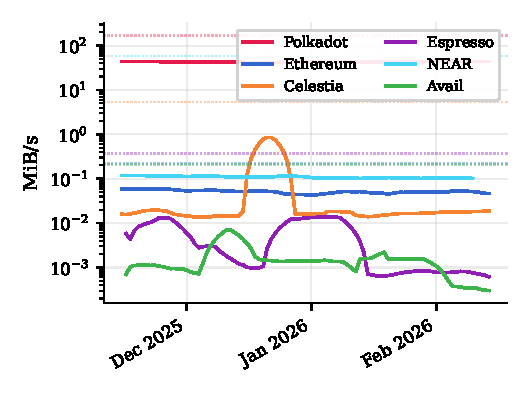
\includegraphics[width=\textwidth]{cross_throughput.pdf}
        \caption{Throughput (MiB/s, 7-day mean, log scale)}
    \end{subfigure}\hfill
    \begin{subfigure}[b]{0.49\textwidth}
        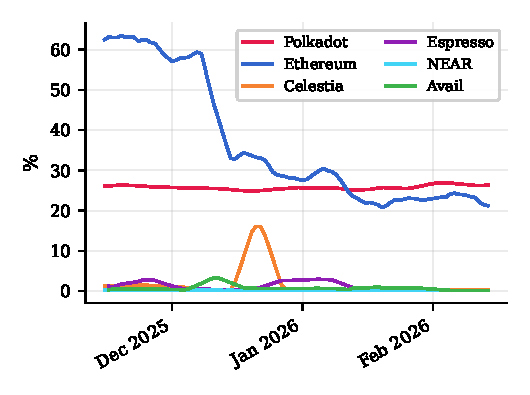
\includegraphics[width=\textwidth]{cross_utilization.pdf}
        \caption{Utilization (\%, 7-day mean)}
    \end{subfigure}

    \vspace{0.2cm}
    \begin{subfigure}[b]{0.49\textwidth}
        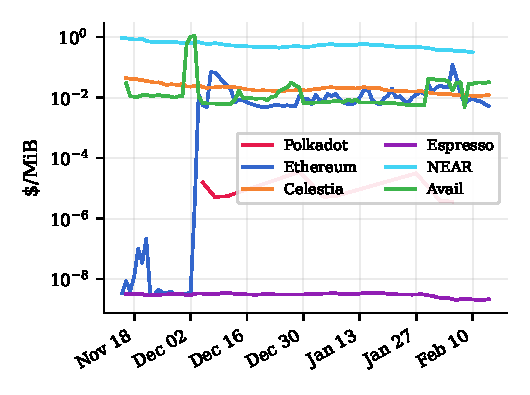
\includegraphics[width=\textwidth]{cross_cost.pdf}
        \caption{Median cost (\$/MiB, log scale)}
    \end{subfigure}\hfill
    \begin{subfigure}[b]{0.49\textwidth}
        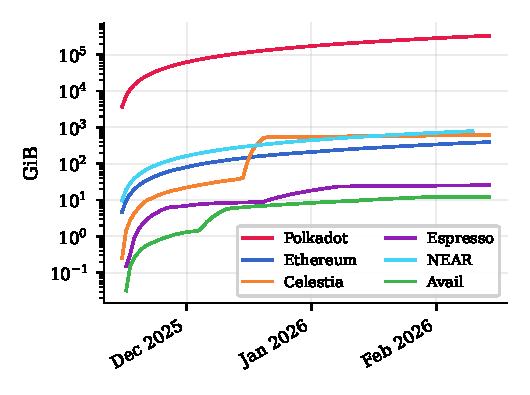
\includegraphics[width=\textwidth]{cross_cumulative.pdf}
        \caption{Cumulative volume (GiB, log scale)}
    \end{subfigure}
    \caption{Cross-protocol comparison over the 90-day window.
    All protocols operate well below their capacity ceilings; Celestia's December~16--21 surge peaks at $\sim$22\% of its (quadrupled) capacity.
    Polkadot throughput and volume are upper bounds (Section~\ref{sec:meth-normalization}).}
    \label{fig:cross}
\end{figure*}

\begin{table}[t]
\centering
\caption{90-day throughput and utilization summary.}
\label{tab:throughput_summary}
\setlength{\tabcolsep}{3pt}
\footnotesize
\begin{tabular}{lcccc}
\toprule
\textbf{Protocol} & \textbf{Max MiB/s} & \textbf{p50 MiB/s} & \textbf{Mean MiB/s} & \textbf{Mean util.} \\
\midrule
Polkadot & $\sim$167 & $\sim$42.8$^\dagger$ & $\sim$43.0$^\dagger$ & $\sim$25.8\% \\
Ethereum & 0.22 & $\sim$0.051 & $\sim$0.051 & $\sim$35\% \\
Celestia & 1.33$\to$5.31 & $\sim$0.018 & $\sim$0.024 & $\sim$1.7\% \\
Espresso & 0.37 & $\sim$0.002 & $\sim$0.003 & $\sim$1.5\% \\
NEAR & $\sim$59 & $\sim$0.107 & $\sim$0.108 & $\sim$0.18\% \\
Avail & 0.21 & $\sim$0.001 & $\sim$0.002 & $<$1\% \\
\bottomrule
\end{tabular}

\vspace{2pt}
\raggedright\footnotesize{$^\dagger$Upper bound: assumes max PoV size per included candidate. Ethereum and Celestia utilization is against the maximum in force on each day.}
\end{table}

Key observations:
\begin{enumerate}
    \item \textbf{Universal under-utilization.} No protocol's mean utilization exceeds 40\%. Polkadot is stable at $\sim$25--27\% ($\sim$26 of 100 cores engaged per day). Ethereum has the highest sustained utilization: $\sim$60\% under Pectra and Fusaka, falling to $\sim$31\% after BPO1 and $\sim$23\% after BPO2 as capacity grew faster than demand. Celestia runs at $\le$1\% in steady state, NEAR at $\sim$0.18\% despite $\sim$9~GiB/day of payload, and Espresso and Avail at a few percent at most.
    \item \textbf{Demand, not supply.} Because all protocols are demand-constrained, observed throughput reflects ecosystem adoption rather than engineering limits; raw MiB/s comparisons measure market share, not capability.
    \item \textbf{NEAR's volume paradox.} NEAR has the lowest utilization but the second-highest volume ($\sim$833~GiB over the window, after Polkadot's upper-bound $\sim$340~TiB; Ethereum $\sim$392~GiB; Celestia $\sim$200~GiB), because its $\sim$59~MiB/s capacity across 9~shards far exceeds demand.
\end{enumerate}

\subsection{Cost Analysis}
\label{sec:results-cost}

Fig.~\ref{fig:cost_quantiles} shows per-protocol daily cost quantile bands (p10/p50/p90) and Table~\ref{tab:cost_summary} summarizes the distributions.

\begin{figure*}[t]
    \centering
    \begin{subfigure}[b]{0.32\textwidth}
        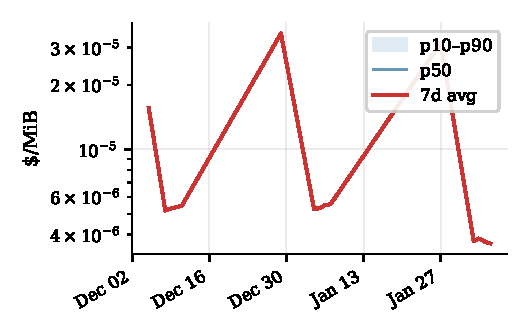
\includegraphics[width=\textwidth]{polkadot_cost.pdf}
        \caption{Polkadot}
    \end{subfigure}\hfill
    \begin{subfigure}[b]{0.32\textwidth}
        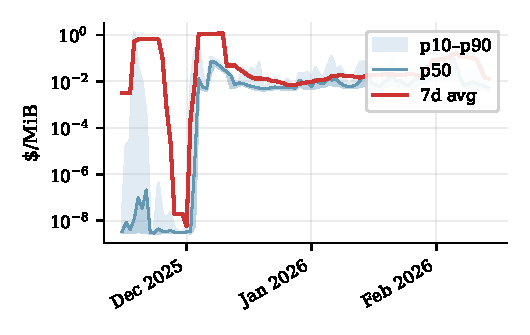
\includegraphics[width=\textwidth]{eth_cost.pdf}
        \caption{Ethereum}
        \label{fig:cost_q_eth}
    \end{subfigure}\hfill
    \begin{subfigure}[b]{0.32\textwidth}
        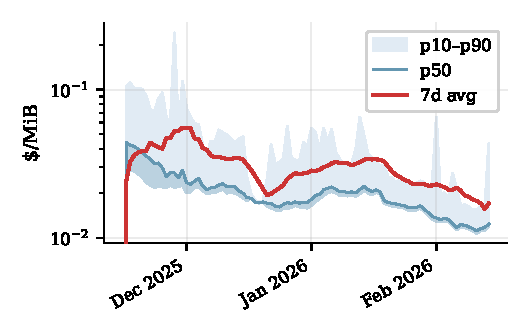
\includegraphics[width=\textwidth]{celestia_cost.pdf}
        \caption{Celestia}
    \end{subfigure}

    \vspace{0.2cm}
    \begin{subfigure}[b]{0.32\textwidth}
        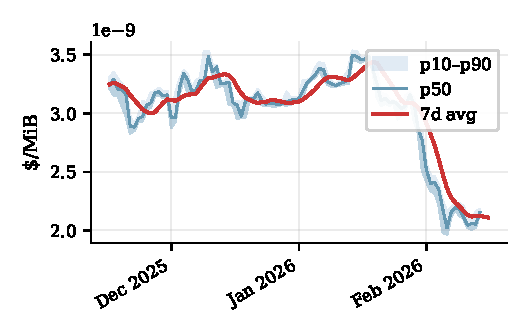
\includegraphics[width=\textwidth]{espresso_cost.pdf}
        \caption{Espresso}
    \end{subfigure}\hfill
    \begin{subfigure}[b]{0.32\textwidth}
        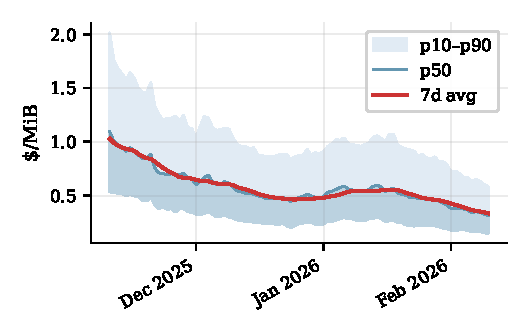
\includegraphics[width=\textwidth]{near_cost.pdf}
        \caption{NEAR}
    \end{subfigure}\hfill
    \begin{subfigure}[b]{0.32\textwidth}
        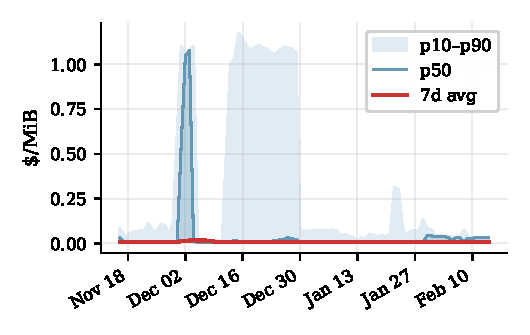
\includegraphics[width=\textwidth]{avail_cost.pdf}
        \caption{Avail}
    \end{subfigure}
    \caption{Daily cost quantile bands (\$/MiB) per protocol.
    (a)~Polkadot bulk coretime, on days with purchases only.
    (b)~Ethereum: fees sit at the 1-wei floor until Fusaka (Dec~3), then settle near \$0.005--0.02/MiB.
    (c)~Celestia declines from $\sim$\$0.05 to $\sim$\$0.02/MiB, partly with the TIA price.
    (d)~Espresso's fixed 1~wei/byte fee tracks ETH/USD.
    (e)~NEAR has the highest median among active fee markets.
    (f)~Avail has the widest spread, with p50 spikes above \$1/MiB.}
    \label{fig:cost_quantiles}
\end{figure*}

\begin{table}[t]
\centering
\caption{90-day cost summary (\$/MiB).}
\label{tab:cost_summary}
\setlength{\tabcolsep}{2.5pt}
\footnotesize
\begin{tabular}{lccccc}
\toprule
\textbf{Protocol} & \textbf{p50} & \textbf{p90} & \textbf{p99} & \textbf{VWAP} & \textbf{Pricing} \\
\midrule
Polkadot & 5.3$\times$10$^{-6}$$^\ast$ & 2.7$\times$10$^{-5}$ & 3.5$\times$10$^{-5}$ & --- & Coretime \\
Ethereum & 7.3$\times$10$^{-3}$ & 0.023 & 0.074 & 0.18 & Blob gas \\
Celestia & 0.020 & 0.030 & 0.042 & 0.025 & Gas/byte \\
Espresso & 3.1$\times$10$^{-9}$ & 3.4$\times$10$^{-9}$ & 3.5$\times$10$^{-9}$ & 3.1$\times$10$^{-9}$ & Fixed fee \\
NEAR & 0.53 & 0.71 & 0.92 & 0.54 & Gas \\
Avail & 0.0096 & 0.032 & 1.05 & 0.0074 & Fee+modifier \\
\bottomrule
\end{tabular}

\vspace{2pt}
\raggedright\footnotesize{$^\ast$Sparse: 14 of 94 days had bulk coretime purchases; amortized over max PoV capacity. Quantiles are over the distribution of daily median costs in the window for every protocol; VWAP is total DA spend divided by total DA volume.}
\end{table}

Key findings:
\begin{enumerate}
    \item \textbf{More than eight orders of magnitude.} Median DA cost ranges from $\sim$\$3$\times$10$^{-9}$/MiB (Espresso) to $\sim$\$0.53/MiB (NEAR). The range reflects different economic designs, not only protocol efficiency.
    \item \textbf{Espresso's cost is not an economic signal.} The fee has been fixed at 1~wei/byte since genesis, so its curve mirrors ETH/USD (falling from $\sim$\$3.5$\times$10$^{-9}$ to $\sim$\$2$\times$10$^{-9}$ as ETH fell). This is a permissioned Mainnet~0 artifact, not a fee market.
    \item \textbf{Ethereum's floor exit is driven by EIP-7918, not by BPO demand.} Before Fusaka the blob base fee sat at the 1-wei floor for $\sim$28\% of blocks and the median cost was $\sim$\$4$\times$10$^{-9}$/MiB. From the first post-Fusaka day the floor share drops to zero and median cost jumps six orders of magnitude to $\sim$\$0.009/MiB, before BPO1 adds any capacity (Section~\ref{sec:results-upgrades}).
    \item \textbf{Avail has the widest spread.} Its median (\$0.0096/MiB) is comparable to Celestia's, but its p99 reaches $\sim$\$1.05 during brief activity surges around December~4 and late December, suggesting the fee modifier amplifies volatility even at low throughput.
    \item \textbf{NEAR has the highest meaningful cost}, declining from $\sim$\$0.75 to $\sim$\$0.30/MiB over the window, reflecting gas pricing applied to encoded receipt data.
    \item \textbf{Polkadot's cost is sparse but negligible}, because coretime bundles execution and DA; the DA component is effectively a by-product of core acquisition.
\end{enumerate}

\subsubsection{Retention-Adjusted Cost}
Table~\ref{tab:annualized_cost} and Fig.~\ref{fig:landscape}(b) normalize cost by retention (Section~\ref{sec:meth-metrics}).

\begin{table}[t]
\centering
\caption{Annualized DA cost, accounting for retention.}
\label{tab:annualized_cost}
\setlength{\tabcolsep}{4pt}
\begin{tabular}{lccc}
\toprule
\textbf{Protocol} & \textbf{Retention} & \textbf{Reposts/yr} & \textbf{p50 \$/MiB/yr} \\
\midrule
NEAR & $\sim$1.5\,d & $\sim$243 & $\sim$129 \\
Celestia & 7\,d & $\sim$52 & $\sim$1.0 \\
Ethereum & $\sim$18\,d & $\sim$20 & $\sim$0.15 \\
Polkadot & 25\,h & $\sim$350 & $\sim$0.002 \\
Avail & node-set & --- & (spot 0.0096) \\
Espresso & node-set & --- & (spot 3$\times$10$^{-9}$) \\
\bottomrule
\end{tabular}
\end{table}

Short retention multiplies cost: NEAR's 5-epoch garbage-collection window ($\sim$1.5~days) requires $\sim$243 reposts per year and gives by far the highest annualized cost ($\sim$\$129/MiB/yr), while Celestia's 7-day sampling window lifts its \$0.02/MiB spot cost to $\sim$\$1/MiB/yr.
Ethereum's 18-day window keeps its annualized cost near \$0.15/MiB/yr, and Polkadot's cost stays negligible even after $\sim$350 reposts.
Avail and Espresso define no protocol-level expiry, so their cost cannot be annualized on the same basis.

\begin{figure*}[t]
    \centering
    \begin{subfigure}[b]{0.49\textwidth}
        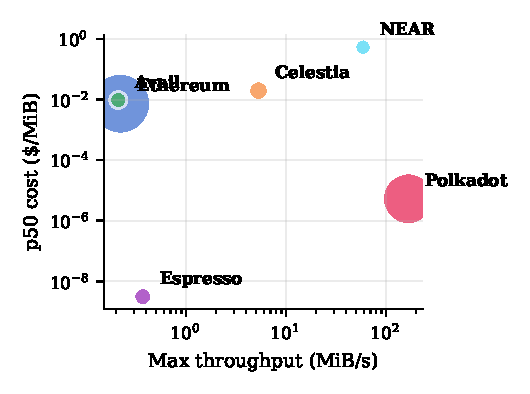
\includegraphics[width=\textwidth]{cross_capacity_vs_cost.pdf}
        \caption{Maximum throughput vs.\ median cost (bubble size: mean utilization)}
    \end{subfigure}\hfill
    \begin{subfigure}[b]{0.49\textwidth}
        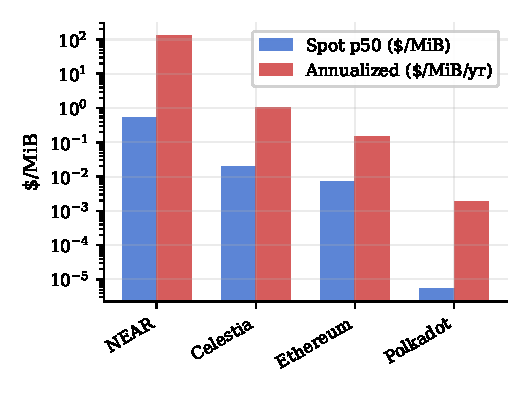
\includegraphics[width=\textwidth]{cross_retention_adjusted_cost.pdf}
        \caption{Spot vs.\ annualized cost}
    \end{subfigure}
    \caption{DA protocol landscape. Protocols cluster by design philosophy rather than along a single capacity--cost frontier, and retention reorders the cost ranking.}
    \label{fig:landscape}
\end{figure*}

\subsection{Natural Experiments: Protocol Upgrades}
\label{sec:results-upgrades}

\subsubsection{Ethereum: Pectra $\rightarrow$ Fusaka $\rightarrow$ BPO1 $\rightarrow$ BPO2}

Fig.~\ref{fig:eth} separates the effect of Ethereum's three upgrades.
\squishlist
    \item \textbf{Fusaka (fee floor).} Under Pectra the blob fee was at the 1-wei minimum for 5--68\% of blocks per day. Fusaka's EIP-7918 ties a reserve price to the execution base fee; from December~4 no block is at the floor (Fig.~\ref{fig:eth}(c)) and median cost rises to $\sim$\$0.009/MiB, while utilization is unchanged ($\sim$58\%).
    \item \textbf{BPO1 and BPO2 (capacity).} Each capacity step lowered utilization (from $\sim$58\% to $\sim$31\% to $\sim$23\%) and target utilization (from $\sim$87\% to $\sim$47\% to $\sim$34\%; Fig.~\ref{fig:eth}(b)). Median cost stayed in a narrow \$0.007--0.010/MiB band across both BPO eras (Fig.~\ref{fig:eth}(a)), consistent with fees held near the EIP-7918 reserve price rather than set by congestion.
    \item \textbf{Demand.} Daily blob volume stayed at $\sim$4.1--4.7~GiB/day across all four eras, so the added capacity has not yet been absorbed.
\squishend

\begin{figure*}[t]
    \centering
    \begin{subfigure}[b]{0.32\textwidth}
        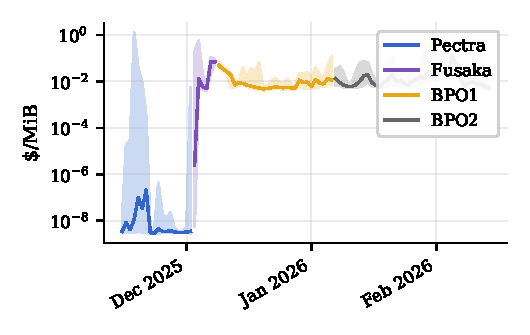
\includegraphics[width=\textwidth]{eth_cost_eras.pdf}
        \caption{Cost bands by era (\$/MiB)}
    \end{subfigure}\hfill
    \begin{subfigure}[b]{0.32\textwidth}
        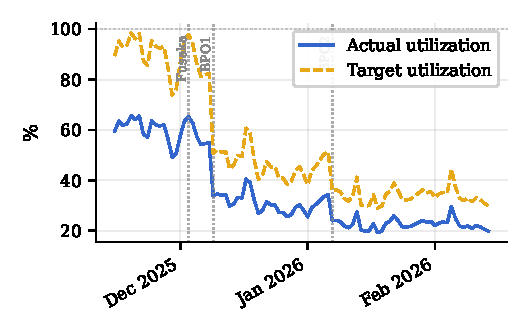
\includegraphics[width=\textwidth]{eth_target_vs_actual.pdf}
        \caption{Target vs.\ actual utilization (\%)}
    \end{subfigure}\hfill
    \begin{subfigure}[b]{0.32\textwidth}
        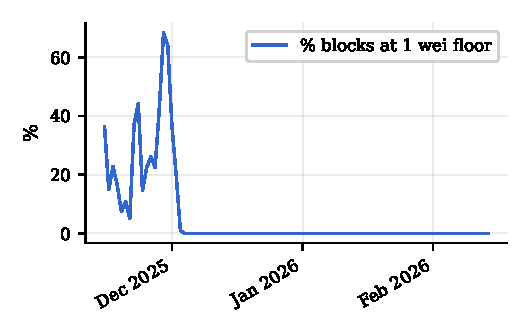
\includegraphics[width=\textwidth]{eth_pct_at_floor.pdf}
        \caption{Blocks at the 1-wei fee floor (\%)}
    \end{subfigure}
    \caption{Ethereum blob market across the Pectra, Fusaka, BPO1 and BPO2 eras. The fee leaves the floor at Fusaka (EIP-7918), before any capacity change; the BPO forks lower utilization without materially changing median cost.}
    \label{fig:eth}
\end{figure*}

\subsubsection{Celestia: December Demand Surge}

Celestia raised its maximum square from 128 to 256 on December~3, quadrupling capacity to $\sim$5.3~MiB/s.
From December~16 to~21, daily throughput rose eighty-fold, from a baseline of $\sim$0.015~MiB/s to $\sim$1.2~MiB/s. That is $\sim$22\% of the new ceiling, but it would have saturated the pre-December capacity of 1.33~MiB/s.
Cost did \emph{not} rise: the daily median fell slightly (\$0.020 to \$0.017/MiB) and the p90 collapsed onto the median, indicating that the surge consisted of large blobs posted at the minimum gas price rather than competing demand. Afterwards throughput and the p90 returned to their pre-event levels.
The episode shows capacity being added ahead of demand: the largest demand event in our window did not exercise the fee market.

\subsection{Block Dynamics and Polkadot Core Engagement}
\label{sec:results-blocks}

Fig.~\ref{fig:blocks}(a--b) shows block time distributions for the two protocols where they are informative; fixed-cadence protocols (Ethereum 12\,s, Polkadot 6\,s, Avail 20\,s) are trivially tight.
Celestia holds 5--6\,s after an elevated p90 in mid-November.
Espresso's responsive HotShot consensus has p10~$\sim$1\,s and p50~$\sim$2\,s, with a p90 that falls from $\sim$6.5\,s in the first weeks to $\sim$3\,s by February.

Fig.~\ref{fig:blocks}(c) shows that only $\sim$26 of 100 Polkadot cores were engaged on a typical day, leaving $\sim$74\% idle capacity: the relay chain could host roughly three times as many parachains at current PoV sizes without parameter changes.

\begin{figure*}[t]
    \centering
    \begin{subfigure}[b]{0.32\textwidth}
        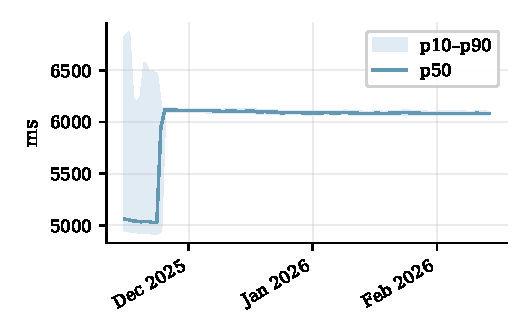
\includegraphics[width=\textwidth]{celestia_blocktime.pdf}
        \caption{Celestia block time (ms)}
    \end{subfigure}\hfill
    \begin{subfigure}[b]{0.32\textwidth}
        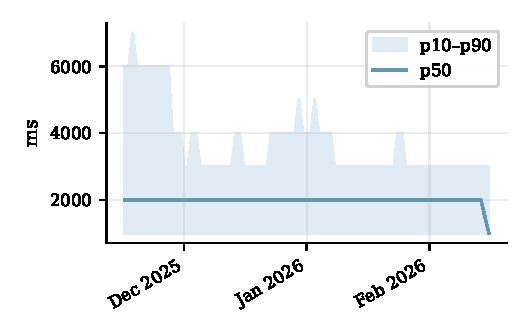
\includegraphics[width=\textwidth]{espresso_blocktime.pdf}
        \caption{Espresso block time (ms)}
    \end{subfigure}\hfill
    \begin{subfigure}[b]{0.32\textwidth}
        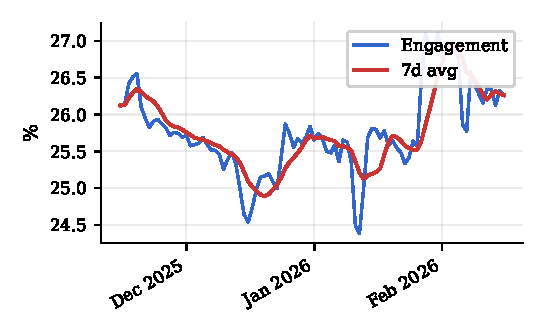
\includegraphics[width=\textwidth]{polkadot_core_engagement.pdf}
        \caption{Polkadot core engagement (\%)}
    \end{subfigure}
    \caption{Block time distributions (p10/p50/p90) for Celestia and Espresso, and Polkadot core engagement.}
    \label{fig:blocks}
\end{figure*}

Espresso's payload pattern (two burst periods in November and late December--early January, then collapse to $<$50~MiB/day) suggests non-organic traffic typical of an early permissioned deployment, in contrast to Celestia's sustained 30--100~MiB/hour baseline.
